\documentclass[12pt]{article}
\usepackage{tikz}

\begin{document}

\begin{center}
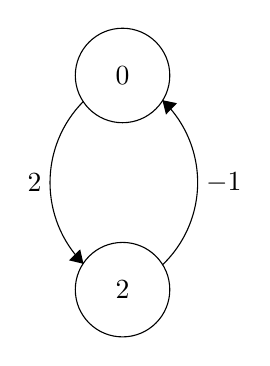
\begin{tikzpicture}[scale=0.2]
\tikzstyle{every node}+=[inner sep=0pt]
\draw [black] (35.6,-19.7) circle (3);
\draw (35.6,-19.7) node {$0$};
\draw [black] (35.6,-33.3) circle (3);
\draw (35.6,-33.3) node {$2$};
\draw [black] (33.116,-31.655) arc (-135.24857:-224.75143:7.322);
\fill [black] (33.12,-31.66) -- (32.91,-30.74) -- (32.2,-31.44);
\draw (30.49,-26.5) node [left] {$2$};
\draw [black] (38.132,-21.269) arc (46.32422:-46.32422:7.232);
\fill [black] (38.13,-21.27) -- (38.36,-22.18) -- (39.06,-21.46);
\draw (40.87,-26.5) node [right] {$-1$};
\end{tikzpicture}
\end{center}

\end{document}
